\scanpage{106}
\diagram{\begin{tikzcd}[column sep=huge,row sep=huge]
K^-_{\unsure{fini}}(K)^\circ\arrow[r,"D"]\arrow[d,"T"']
\arrow[dr,phantom,"\substack{\uline{\text{Théorie de}}\\\uline{\text{dualité gén.}}\quad\simeq}"]&
K^+_{\unsure{fini}}(K)\arrow[d,"T(-1)"]\\
K^-(k)'{}^\circ\arrow[r,dash,"\Delta"]\arrow[d,"S"']
\arrow[dr,phantom,"\substack{\uline{\text{Frobenius}}\\\uline{\text{-Lang}}\quad\simeq}"]&
K^+(k)'\arrow[d,"S(-1)"]\\
K^-\deleted{\unsure{\mathcal G}}\mathcal C^\circ\arrow[r,"\Theta"]&K^+\mathcal C
\end{tikzcd}}
\[
\left\{\begin{array}{ll}
D&\text{dualité de Cartier}\\
\Delta&\text{dualité de Serre}\\
\Theta&\text{dualité de \unsure{Pontryagin}}
\end{array}\right.
\]
$\mathcal C$ groupes top. abéliens loc. compacts tt discontinus

(le $'$ indique qu'on n'admet pas de composantes $\mathbb Z$)

$k$ corps \uuline{fini}
\[
\left\{\begin{array}{ll}
T&\text{foncteur Greenberg-\unsure{Néron}-Grothendieck}\\
S&\text{foncteur }\Gamma_k
\end{array}\right.
\]
Comment obtient on le carré du bas ?

\deleted{\unsure{Remarque}}
\diagram{\begin{tikzcd}[column sep=small,row sep=small]
\operatorname{Ext}^i_{k\text{gr}}(G,\mathbb Z/n\mathbb Z)\arrow[r,equal,"\sim"]&
\operatorname{Ext}^{i-1}_{\mathrm{gr.top.}}(SG,\mathbb Z/n\mathbb Z)\arrow[d,equal]\\
&\operatorname{Ext}^i(SG,\mathbb Z/n\mathbb Z(-1))
\end{tikzcd}}
\diagram{\begin{tikzcd}
G\arrow[r,"\text{deg }i"]&\mathbb Z/n\mathbb Z
\end{tikzcd}}
\diagram{\begin{tikzcd}
SG\arrow[r,"\text{deg }i"]&S(\mathbb Z/n\mathbb Z)\arrow[r,"\text{degré }0"]&
\mathbb Z/n\mathbb Z(-1)
\end{tikzcd}}
\[
\begin{aligned}
\underline{\underline{\operatorname{Ext}}}^{0}_{\mathrm{gr.top}}
(\unsure{S(\mathbb Z/n\mathbb Z)|\{\mathbb Z/n\mathbb Z\}}\deleted{(-1)},\mathbb Z/n\mathbb Z(-1))
&=\underline{\underline{\operatorname{Ext}}}^{-1}_{k\mathrm{gr}}
(S(\mathbb Z/n\mathbb Z),\mathbb Z/n\mathbb Z)\\
&=\operatorname{Hom}(H^{\unsure{1}}S(\mathbb Z/n\mathbb Z),\mathbb Z/n\mathbb Z)
\simeq\mathbb Z/n\mathbb Z\quad !
\end{aligned}
\]
\margin{\figure{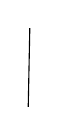
\begin{tikzpicture}\draw (0,0)--(.02,1);\end{tikzpicture}}}
\deleted{$\unsure{\mathbb Z}$}
\mspage{105}

